\documentclass[12pt,letterpaper]{hmcpset}
\usepackage[margin=1in]{geometry}
\usepackage{graphicx}

% info for header block in upper right hand corner
\name{Box number: \underline{\hspace{1cm}} (name on back) }
\class{Math 60: Section \underline{\hspace{1cm}}}
\assignment{Assignment 5}
\duedate{Due Date: 10/12/18}

\begin{document}

\problemlist{
Section 5.2: 7, 14\\
Section 5.3: 1, 13, 18\\
Section 5.4: 4, 5\\
Section 5.5: 9, 20, 25, 31, 34, 38
}

\begin{problem}
Section 5.2 \#7. In Exercises 4-13, evaluate the given iterated integrals. In addition, sketch the regions $D$ that are determined by the limits of integration.
$$ \int_{-1}^{3} \int_{x}^{2x+1} x y \,dy \,dx $$
\end{problem}

\newpage

\begin{problem}
Section 5.2 \#14. Figure 5.43 shows the level curves indicating the varying depth (in feet) of a $25$ ft by $50$ ft swimming pool. Use a Riemann sum to estimate, to the nearest $100$ ft$^3$, the volume of water that the pool contains.
\begin{center}
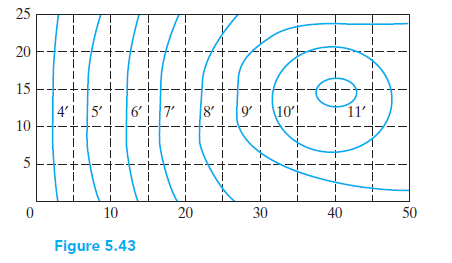
\includegraphics[width=0.5\textwidth]{figure5-43.png}
\end{center}
\end{problem}

\newpage

\begin{problem}
Section 5.3 \#1. Consider the integral
$$ \int_{0}^{2} \int_{x^2}^{2x} (2x+1) \,dy \,dx .$$
\begin{enumerate}
	\item[(a)] Evaluate this integral.
	\item[(b)] Sketch the region of integration.
	\item[(c)] Write an equivalent iterated integral with the order of integration reversed. Evaluate this new integral and check that your answer agrees with part (a).
\end{enumerate}
\end{problem}

\newpage

\begin{problem}
Section 5.3 \#13. In Exercises 12 and 13, rewrite the given sum of iterated integrals as a single iterated integral by reversing the order of integration, and evaluate.
$$ \int_{0}^{8} \int_{0}^{\sqrt{y/3}} y \,dx \,dy + \int_{8}^{12} \int_{\sqrt{y-8}}^{\sqrt{y/3}} y \,dx \,dy.$$
\end{problem}

\newpage

\begin{problem}
Section 5.3 \#18. In Exercises 14-18, evaluate the given iterated integral.
$$ \int_{0}^{2} \int_{y/2}^{1} e^{-x^2} \,dx \,dy$$
\end{problem}

\newpage

\begin{problem}
Section 5.4 \#4. Find the value of $\iiint_{W} z \,dV$ where $W = [-1, 2] \times [2, 5] \times [-3, 3]$, without resorting to explicit calculation.
\end{problem}

\newpage

\begin{problem}
Section 5.4 \#5. Evaluate the iterated integrals given in Exercises 5-7.
$$ \int_{-1}^{2} \int_{1}^{z^2} \int_{0}^{y+z} 3yz^2 \,dx \,dy \,dz $$
\end{problem}

\newpage

\begin{problem}
Section 5.5 \#9. Evaluate the integral
$$ \int_{0}^{2} \int_{x/2}^{(x/2)+1} x^5 (2y-x) e^{(2y-x)^2} \,dy \,dx $$
by making the substitution $u=x$, $v=2y-x$.
\end{problem}

\newpage

\begin{problem}
Section 5.5 \#20. Find the total area enclosed inside the rose $r = \sin{2 \theta}$. (Hint: Sketch the curve and find the area inside a single leaf.)
\end{problem}

\newpage

\begin{problem}
Section 5.5 \#25. Evaluate
$$ \iint_D \cos{(x^2 + y^2)} \,dA, $$
where $D$ is the shaded region in Figure 5.106.
\begin{center}
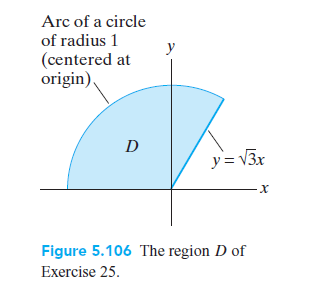
\includegraphics[width=0.5\textwidth]{figure5-106.png}
\end{center}
\end{problem}

\newpage

\begin{problem}
Section 5.5 \#31. Determine
$$ \iiint_W (x^2 + y^2 + 2z^2) \,dV, $$
where $W$ is the solid cylinder represented by the inequalities $x^2 + y^2 \leq 4, -1 \leq z \leq 2$.
\end{problem}

\newpage

\begin{problem}
Section 5.5 \#34. In Exercises 34 and 35, determine the values of the given integrals, where $W$ is the region bounded by the two spheres $x^2 + y^2 + z^2 = a^2$ and $x^2 + y^2 + z^2 = b^2$, for $0 < a < b$.
$$ \iiint_W \frac{\,dV}{\sqrt{x^2 + y^2 + z^2}} $$
\end{problem}

\newpage

\begin{problem}
Section 5.5 \#38. Determine
$$ \iiint_W \left( 2 + \sqrt{x^2 + y^2} \right) \,dV$$
where $W=\{ (x, y, z) | \sqrt{x^2 + y^2} \leq z/2 \leq 3 \}$.
\end{problem}
\end{document}